\documentclass[homework]{IEEEtran}
\IEEEoverridecommandlockouts
% The preceding line is only needed to identify funding in the first footnote. If that is unneeded, please comment it out.
\usepackage{cite}
\usepackage{CJKutf8}
\usepackage{indentfirst}
\usepackage{amsmath,amssymb,amsfonts}
\usepackage{algorithmic}
\usepackage{graphicx}
\usepackage{textcomp}
\usepackage{xcolor}
\usepackage{hyperref}
\usepackage[justification=centering]{caption}
\setlength{\parindent}{2em}
\def\BibTeX{{\rm B\kern-.05em{\sc i\kern-.025em b}\kern-.08em
    T\kern-.1667em\lower.7ex\hbox{E}\kern-.125emX}}
\begin{document}

\title{Semiconductor Material Testing and Analysis II\\
{\footnotesize \textsuperscript{*}Name: Xue Yuan  | Student number: 202228015926034}
}

\author{}
\maketitle

\begin{abstract}
This document is about the second homework for Semiconductor Material Testing and Analysis by \LaTeX.
\end{abstract}

\section{Result of calculate}
\begin{CJK}{UTF8}{gkai}
$\mathbf{Q1}$: 对一半导体材料的电阻率进行了10次的等精度测量,结果如下(单位:$\Omega$⋅/cm): \par
    [25.003,25.013,25.024,25.000,25.010,        \par
    25.030,25.020,25.007,25.027,25.016]         \par
计算:本次测量的算术平均值和标准偏差,并正确表示测量结果。 \par
$\mathbf{A}$: 由算术平均值和标准偏差的定义:
$$
\bar{x}=E(x)=\lim _{n \rightarrow \infty} \frac{1}{n} \sum_{i=1}^{n} x_{i}
$$
$$
s=\left[\frac{1}{n-1}\left(\sum_{i=1}^{n} x_{i}^{2}-n \bar{x}^{2}\right)\right]^{1 / 2}
$$
可以计算:
\begin{figure}[htb]
\centerline{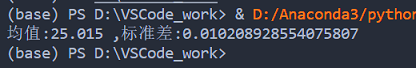
\includegraphics{Images/fig1.png}}
\caption{Program results}
\label{fig1}
\end{figure}
\begin{enumerate}
\item $\bar{x}=25.015$
\item $s=1.0209 \times 10^{-2}$
\end{enumerate}

$\mathbf{Q2}$: 有下列一组测量数据:  \par
    [10.06,10.07,10.06,10.08,10.10,        \par
    10.12,10.14,10.18,10.18,10.21]         \par
采用残差观察法(作图或列表)判断是否有系统误差,若有说明系统误差类型 \par
$\mathbf{A}$: 由残差定义$v_i = x_i - \bar{x}$
\begin{figure}[htb]
\centerline{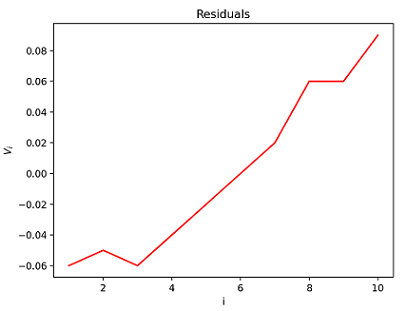
\includegraphics{Images/fig2.jpg}}
\caption{Residual Plot}
\label{fig2}
\end{figure}
可以明显看出,系统存在线性的系统误差。 \par
$\mathbf{Q3}$:对上题中的实验数据,试用马利科夫判据判断是否有线性系统误差的存在。\par
$\mathbf{A}$:由马尔科夫判据的定义:
$$
\Delta=\sum_{i=1}^{k} v_{i}-\sum_{i=k+1}^{n} v_{i}
$$
我们可以编写程序,计算奇数列偶数列的差和值: \par
\begin{figure}[htb]
\centerline{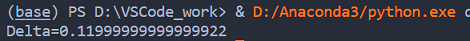
\includegraphics{Images/fig3.png}}
\caption{Malikov's criterion output}
\label{fig3}
\end{figure}
可以看出,$\Delta = 0.12 \gg 0$。综上,我们可以确定数据存在系统误差。 \par
$\mathbf{Q4}$:有如下一组电压测量数据(单位:mV):\par
    [50.74,50.76,50.82,50.85,50.83,      \par
    50.74,50.75,50.81,50.85,50.85]       \par
请分别采用阿贝判据和阿贝-赫梅尼判据判断是否有周期性系统误差的存在。\par
$\mathbf{A}$:由阿贝判据和阿贝-赫梅尼判据的定义:
\begin{enumerate}
\item 阿贝判据: 
$$
C=\frac{1}{n} \sum_{i=1}^{n} v_{i} v_{i+1}>\frac{1}{\sqrt{n}} \sigma^{2}
$$
\item 阿贝-赫梅尼判据: 
$$
n\left|C^{\prime}\right|=\left|\sum_{i=1}^{n-1} v_{i} v_{i+1}\right|>\sqrt{n-1} \sigma^{2}
$$
\end{enumerate}
若满足上式,则可判断列中含有随机误差。   \par
计算结果如下图所示:        \par
\begin{figure}[htb]
\centerline{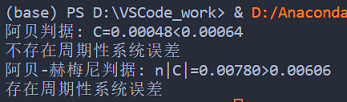
\includegraphics{Images/fig4.png}}
\caption{Program results}
\label{fig4}
\end{figure}
可以看出,使用阿贝判据时,可以判断出体系不存在周期性误差;但使用阿贝-赫梅尼判据
消除最后一项的额外震荡后,反而可以判断出体系存在周期性误差。
\end{CJK}

\section{Appendix}
\begin{CJK}{UTF8}{gkai}
    本次作业中,所采用的拟合计算代码均是基于Matlab和Python3.9,相关的源码已经被开源于Github上:
    \url{https://github.com/Alexiopro/First-year-of-UCAS/tree/main/UCAS/Semiconductor%20Material%20Testing%20and%20Analysi}
    供读者查用。 \par
\end{CJK}

\end{document}
